% This is samplepaper.tex, a sample chapter demonstrating the
% LLNCS macro package for Springer Computer Science proceedings;
% Version 2.20 of 2017/10/04
%
\documentclass[runningheads]{llncs}
\renewcommand{\baselinestretch}{1.1} 
%
\usepackage{graphicx}
\usepackage[table]{xcolor}
\usepackage{xspace}
\usepackage{hyperref}
\usepackage{subcaption}
\usepackage{listings}
\usepackage{ulem}

\usepackage[para,online,flushleft]{threeparttable}
\usepackage{booktabs}
\usepackage{multirow}
% \usepackage{geometry}
% \usepackage{marginnote}

% Fix link colors
\hypersetup{
    colorlinks = true,
    linkcolor=red,
    citecolor=red,
    urlcolor=blue,
    linktocpage % so that page numbers are clickable in toc
}

% Used for displaying a sample figure. If possible, figure files should
% be included in EPS format.
%
% If you use the hyperref package, please uncomment the following line
% to display URLs in blue roman font according to Springer's eBook style:
% \renewcommand\UrlFont{\color{blue}\rmfamily}
\newcommand{\TG}[1]{\noindent{\color{blue}[\textsc{From Tristan:} #1]}\xspace}
\newcommand{\Ali}[1]{\noindent{\color{green}[\textsc{From Ali:} #1]}\xspace}
\newcommand{\GK}[1]{\noindent{\color{purple}[\textsc{From Greg:} #1]}\xspace}
\newcommand{\YC}[1]{\noindent{\color{orange}[\textsc{From Yohan:} #1]}\xspace}
\newcommand{\anonymous}[1]{***\xspace}


\lstdefinestyle{customC}{
  belowcaptionskip=1\baselineskip,
  breaklines=true,
  xleftmargin=\parindent,
  language=C,
  showstringspaces=false,
  basicstyle=\scriptsize\ttfamily,
  keywordstyle=\bfseries\color[rgb]{0.580, 0.000, 0.827},
  %{purple!40!lightgray},
  commentstyle=\textit{\color{green!40!black}},
  identifierstyle=\bfseries\color{cyan!75!black},
  stringstyle=\color{orange},
  deletekeywords={double,float},
  classoffset=1, % starting new class
  otherkeywords={double,float},
  morekeywords={double,float},
  keywordstyle=\bfseries\color{green!55!black},
  classoffset=0
}

\begin{document}

\title{Comparing tool variability and numerical variability in fMRI analyses}

\author{Ali Salari$^1$, Co-authors$^2$, Tristan Glatard$^1$}

\authorrunning{Salari et al.}
% First names are abbreviated in the running head.
% If there are more than two authors, 'et al.' is used.

\institute{$^1$ Anonymous Organization1\\
  $^2$ Anonymous Organization2\\ **@******.***}

\institute{$^1$ Department of Computer Science and Software Engineering, Concordia University\\
  $^2$ Co-authors Organization\\  Montréal, QC, Canada}

\maketitle              % typeset the header of the contribution

\begin{abstract}
abstract\dots

%  \keywords{Computational reproducibility  \and Neuroimaging pipelines \and Monte-Carlo arithmetic.}
\end{abstract}


\section{Introduction}

\begin{description}
  \item[$\bullet$ ] Methodological choice can influence the final determining areas of brain activation. This opens so results flexibility~\cite{bowring2019exploring}. 

  \item[$\bullet$ ] We presented a framework that can investigate the numerical instability of the pipelines based on Monte-Carlo arithmetic
                    by creating a Fuzzy environment, so that instrument mathematical functions implemented in mathematical system libraries (libmath). 

  \item[$\bullet$ ] In this paper, we aim to answer the questions 1) how the fMRI analyses are numerically stable?
                    2) how the numerical variability is in comparison with the tool variability?
\end{description} 


\section{Methodology}

\subsection{libmath Fuzzy System}

\begin{description}
  \item[$\bullet$ ] libmath Fuzzy allows you to study the numerical stability of tools and pipelines. 
  \item[$\bullet$ ] It is based on MCA perturbations so that applies slight noise on floating-point operations.
  \item[$\bullet$ ] It does not need source code modification or recompilation, and simply works using the Linux LD\_PRELOAD environment variable.
  \item[$\bullet$ ] The library call interposition technique enables us to assess the tools that are dynamically linked to the mathematical library.
\end{description} 


\subsection{fMRI analyses \& Dataset}

\begin{description}
  \item[$\bullet$ ] We replicate the fMRI analyses used in~\cite{bowring2019exploring} using the three most popular packages 
                    for fMRI data processing including FSL, AFNI, and SPM. 
                    
  \item[$\bullet$ ] The functional fMRI studies have been chosen for reanalysis with the publicly available data repositories.
                    The used dataset is available at https://openneuro.org/datasets/ds000001.

  \item[$\bullet$ ] For the ds000001 study, 16 healthy adult subjects participated in a balloon analogue risk task over three scanning sessions.
                    This analysis consists of several common processes. A full description of each analysis is included in~\cite{bowring2019exploring}.

  \item[$\bullet$ ] In the original study, a number of preprocessing steps such as motion correction, segmentation, brain extraction, and registration 
                    were applied in all of the analyses to ensure that results from each software package could be compared objectively.
  
\end{description}  


\subsection{Data processing}

\begin{description}
  \item[$\bullet$ Containerization] building Docker images for three of the most popular software packages in neuroimaging including FSL, AFNI, and SPM.
                  We ensured that the software versions and all the requisites for running analyses used in all experiments 
                  are identical to the original study.  

  \item[$\bullet$ Between tool variability] check and confirm that obtained results are perfectly replicated comparing to the original study. 

  \item[$\bullet$ Numerical variability] running 3 MCA samples in each condition using the Fuzzy libmath environment. 
                  The conditions could be varying between tools, software versions, or the instrumented precisions. 
    \begin{description}
      \item[$\ast$ Varying precisions] a) only perturbing maximum precisions (OS-level), p=53 bits for double-precision and p=24 bits for single-precision.
                                       This would help to compare uncertainty between tool variability and numerical instability at the OS-level. 
                                       b) perturbing precisions from p=53 bits to p=1 bits by steps of 2 iteratively. 
                                       This would help to find the most similar uncertainty distribution between tool variability and numerical variability.
    \end{description}
    
  \item[$\bullet$ Image types] the fMRI result images that we are investigating are thresholded and unthresholded of the group level activation maps.

  \item[$\bullet$ Comparison metrics] comparing variabilities statistically by computing correlations between T-statistic values, Dice coefficient, 
                  and the number of significant digits.    
% EC is a means to assess whether only superficial scaling differences (differences by a scale factor over all voxels) 
% are responsible for disparities between pair of images.

  \item[$\bullet$ Configuration table] showing the detail of the configurations used for replicating the fMRI results.
\end{description}


\section{Results}

All scripts and results to create the figures in this section are available on GitHub repository
in \url{https://github.com/ali4006/fuzzy-neurotools}.
Replication of all analyses was visually assessed to be the same as the original findings.
We ensured that fMRI analyses were processed successfully.
In this section, we call the cross-software variation and numerical variation,
between tool (BT) and within tool (WT) variability, respectively. 
The within tool variability shows results among different fuzzy libmath
samples for the specific version of the tools, and it is not within tool versions.


A summary of the statistic values from the group-level (un)thresholded T-statistics is conducted in
Table~\ref{table:pipeline-stats}.
The variability between images in each condition was measured using mean and standard deviation of absolute differences,
and Pearson correlation coefficient.
% Overally, we see that values in between tools are comparable to values in within tool results.
% The distribution of the pairwise differences in T-statistic..
% The standard deviations exceeding 2.0 in magnitude..
% Pairwise correlations ranged from 0.43 to 0.7 for within tool variability..


%%%%%%%%%% Summary of statstics %%%%%%%%
\setlength{\tabcolsep}{10pt}
\begin{table}[h]
    \centering
    \begin{tabular}{cccc|ccc}
        \toprule
        \multirow{2}{*}{} & \multicolumn{3}{c}{Thresholded} & \multicolumn{3}{c}{Unthresholded} \\
        \cmidrule{2-4} \cmidrule{5-7} \\
        {} & Mean diff. & Std. diff. & Corr. & Mean diff. & Std. diff. & Corr.  \\
        \midrule
        \rowcolor{lightgray}
        FSL vs. SPM          &  0.00       & 0.00      & 0.00       & 0.00     & 0.00       & 0.00 \\
        \rowcolor{lightgray}
        FSL vs. AFNI         &  0.00       & 0.00      & 0.00       & 0.00     & 0.00       & 0.00 \\
        \rowcolor{lightgray}
        AFNI vs. SPM         &  0.00       & 0.00      & 0.00       & 0.00     & 0.00       & 0.00 \\
        Fuzzy FSL and SPM    &  0.00       & 0.00      & 0.00       & 0.00     & 0.00       & 0.00 \\
        Fuzzy FSL and AFNI   &  0.00       & 0.00      & 0.00       & 0.00     & 0.00       & 0.00 \\
        Fuzzy AFNI and SPM   &  0.00       & 0.00      & 0.00       & 0.00     & 0.00       & 0.00 \\
        \bottomrule
    \end{tabular}
    \caption{Summary of T-statistics mean and standard deviation of differences and correlations of each pair of tools.}
    \label{table:pipeline-stats}
\end{table}


% \subsection{Comparing disparity in BT and WT}
\subsection{Spatial localization of disparity in BT and WT}
% Fig message: showing the magnitude of differences and correlated area
% Fig message: showing numerically dependent parts of the brain


Comparisons of standard deviations between results in WT and BT
on the brain surface are shown in Figure~\ref{fig:thresh-varmaps} and Figure~\ref{fig:unthresh-varmaps}.
Figure~\ref{fig:thresh-varmaps} shows maps for group-level thresholded T-statistics, and
Figure~\ref{fig:unthresh-varmaps} shows maps for group-level unthresholded T-statistic values.
While we observe substantial variations in BT (average std. dev. $\approx$ 1.5),
the order of magnitude of variations in WT is much lower (average std. dev. $\approx$ 0.5),
as was anticipated. However, numerical variability is still significant in WT results.
Moreover, we see the same order of magnitude in WT variations compared to BT variations
in some regions in the thresholded images.
For instance, we see the temporal lobe in anterior view for almost all pairs and the fusiform gyrus in inferior view
for the pairs of FSL-SPM and FSL-AFNI in Figure~\ref{fig:unthresh-varmaps}
that are perfectly replicated using the numerical perturbations. 
Although the unthresholded statistic maps from our analyses also show a different magnitude of
the order of variations in both conditions, std. dev. ranges from $\approx$ 0.12 to $\approx$ 0.5 on average in WT and BT;
there is great comparability between results.
Generally, we obtained more uncertainty on thresholded results, probably due to different thresholding
methods used in different tools.
This can raise further investigations on the thresholding techniques toward stability.


%%%%%%%%%% Var. of Thresh %%%%%%%%
\begin{figure}[b]
  \fbox{\begin{minipage}{\dimexpr \textwidth-2\fboxsep-2\fboxrule}
  \begin{subfigure}[t]{\linewidth}
    \centering
    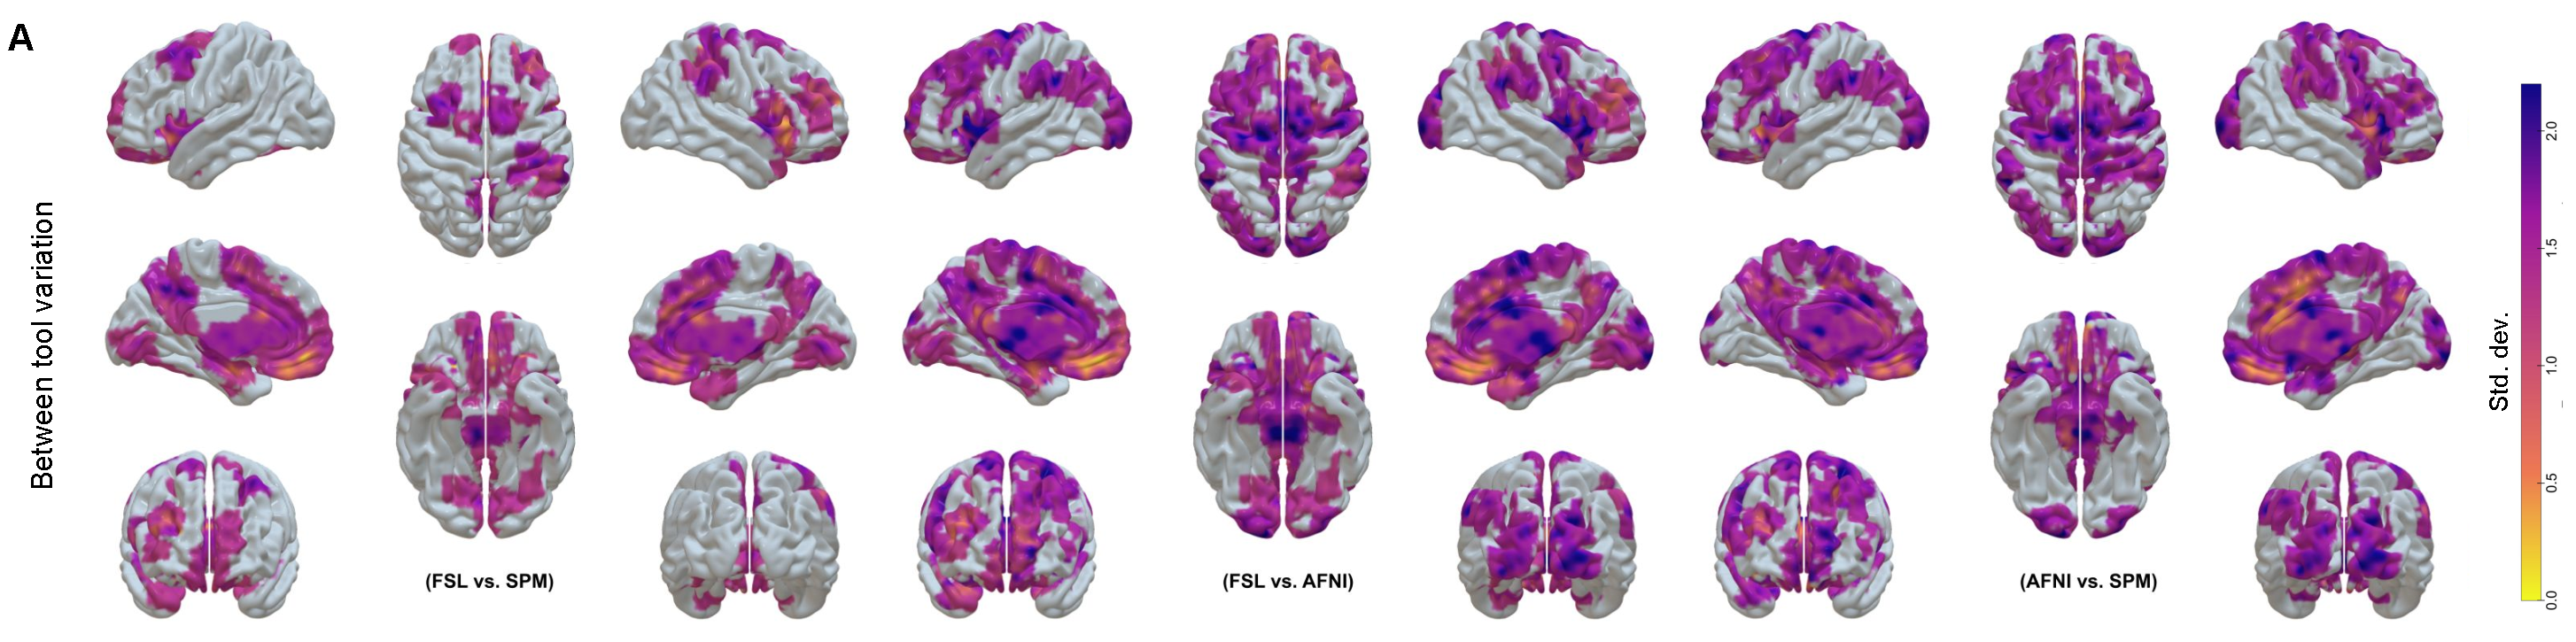
\includegraphics[width=\linewidth]{figures/maps-on-surf-thresh-tool(std).pdf}
    %\caption{Standard deviation of thresholded t-statistics map on template surface}
    \label{fig:thresh-varmaps1}
  \end{subfigure}
  \hfill
  \begin{subfigure}[t]{\linewidth}
    \centering
    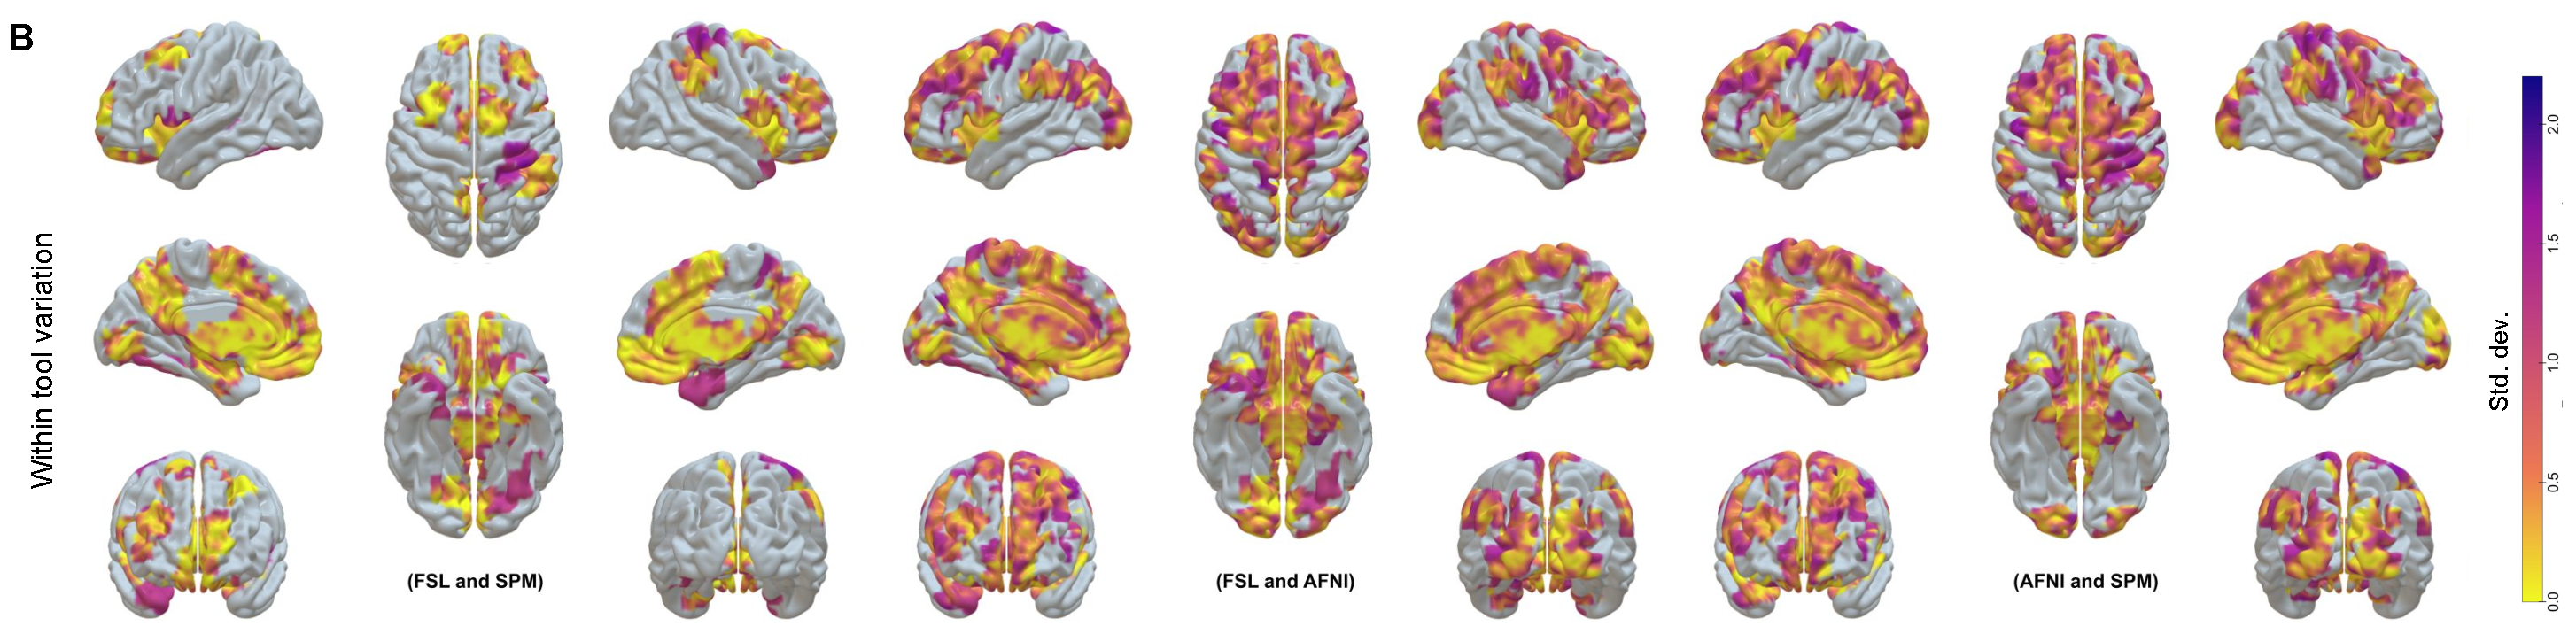
\includegraphics[width=\linewidth]{figures/maps-on-surf-thresh-fuzzy(std).pdf}
    %\caption{Standard deviation of thresholded t-statistics map on template surface}
    \label{fig:thresh-varmaps2}
  \end{subfigure}
  \hfill
  \begin{subfigure}[t]{\linewidth}
    \centering
    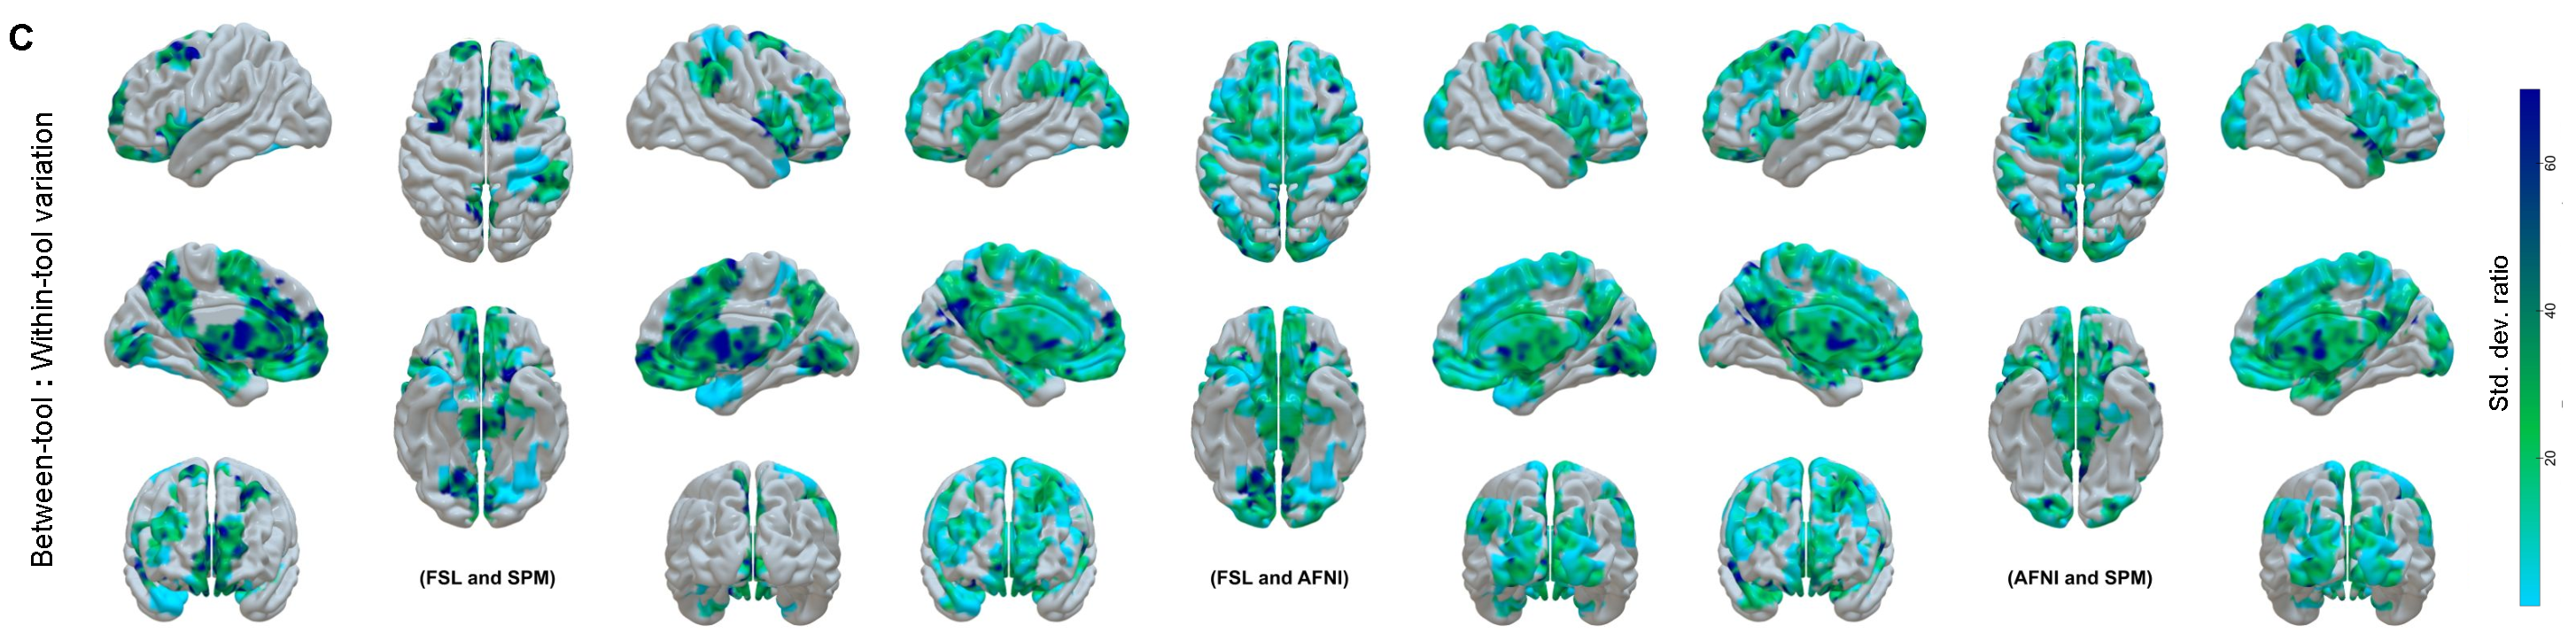
\includegraphics[width=\linewidth]{figures/maps-on-surf-thresh-ratio(std).pdf}
    %\caption{Standard deviation of thresholded t-statistics map on template surface}
    \label{fig:thresh-ratio}
  \end{subfigure}
  \caption{Surface maps of standard deviation of thresholded T-statistics. First and second rows show
  results on between-tool and within-tool results, respectively. Third row represents the ratio of differences
  in between and within tools so that brigher areas indicate more similar order of magnitude of variations in both conditions,
  and vise versa for the darkder regions.}
  \label{fig:thresh-varmaps}
  \end{minipage}}
\end{figure}


%%%%%%%%%% Var. of Unthresh %%%%%%%%
\begin{figure}[b]
  \fbox{\begin{minipage}{\dimexpr \textwidth-2\fboxsep-2\fboxrule}
  \begin{subfigure}[t]{\linewidth}
    \centering
    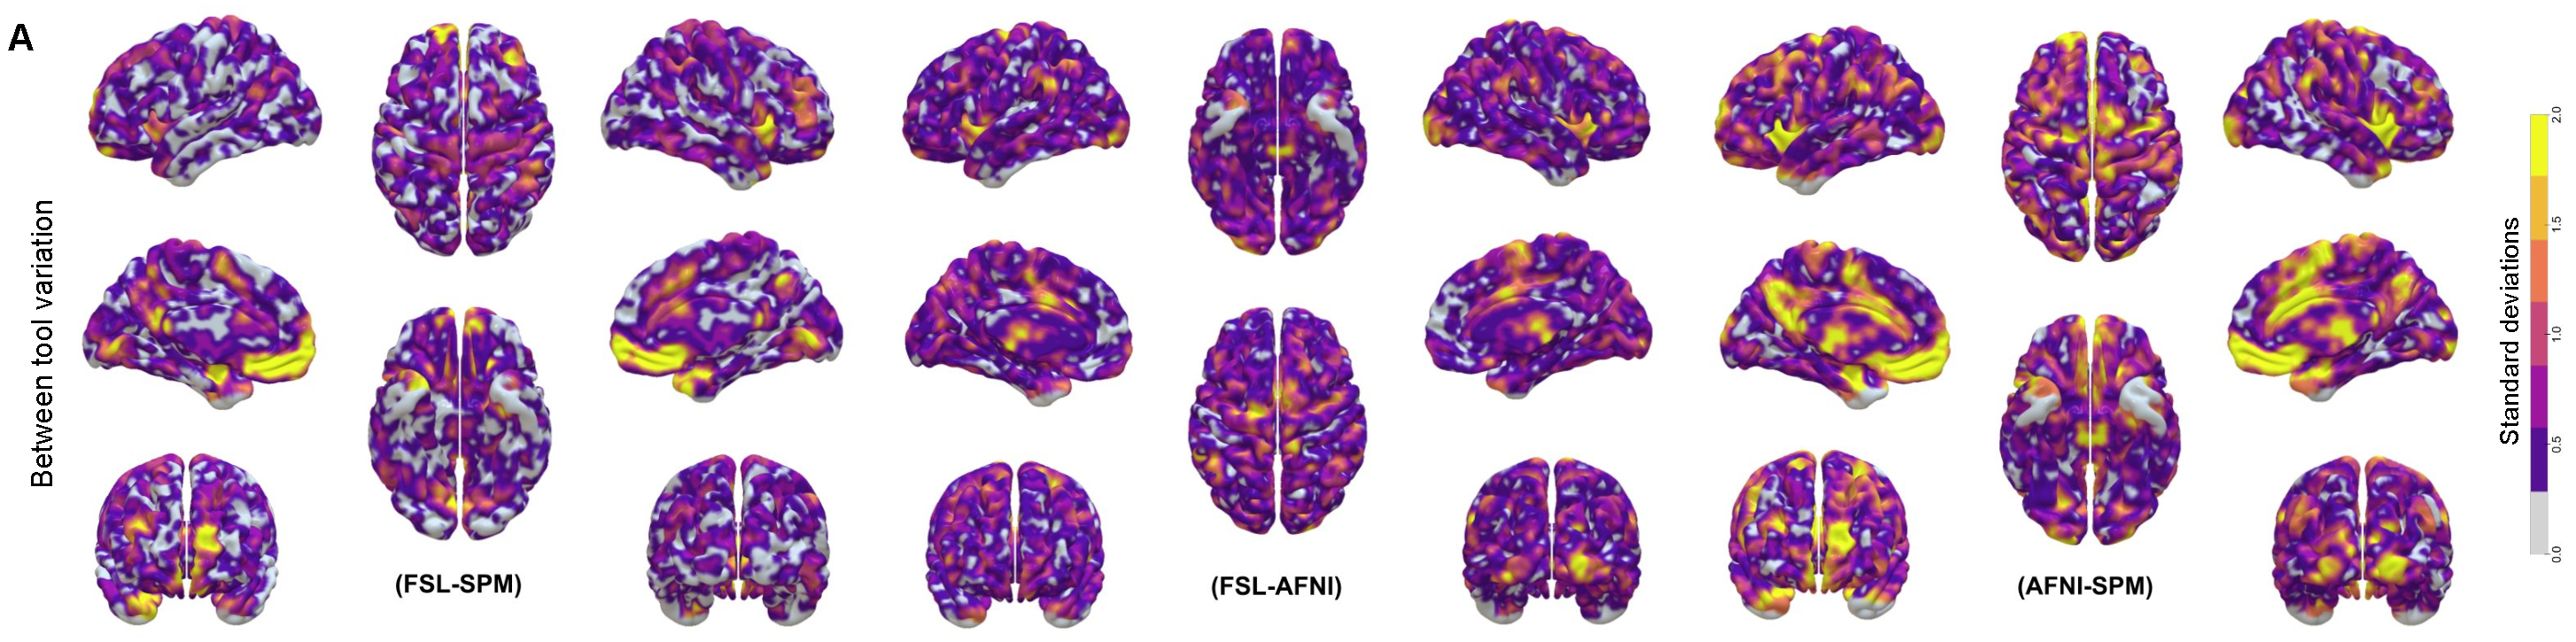
\includegraphics[width=\linewidth]{figures/maps-on-surf-unthresh-tool(std).pdf}
    %\caption{Standard deviation of thresholded t-statistics map on template surface}
    \label{fig:unthresh-varmaps1}
  \end{subfigure}
  \hfill
  \begin{subfigure}[t]{\linewidth}
    \centering
    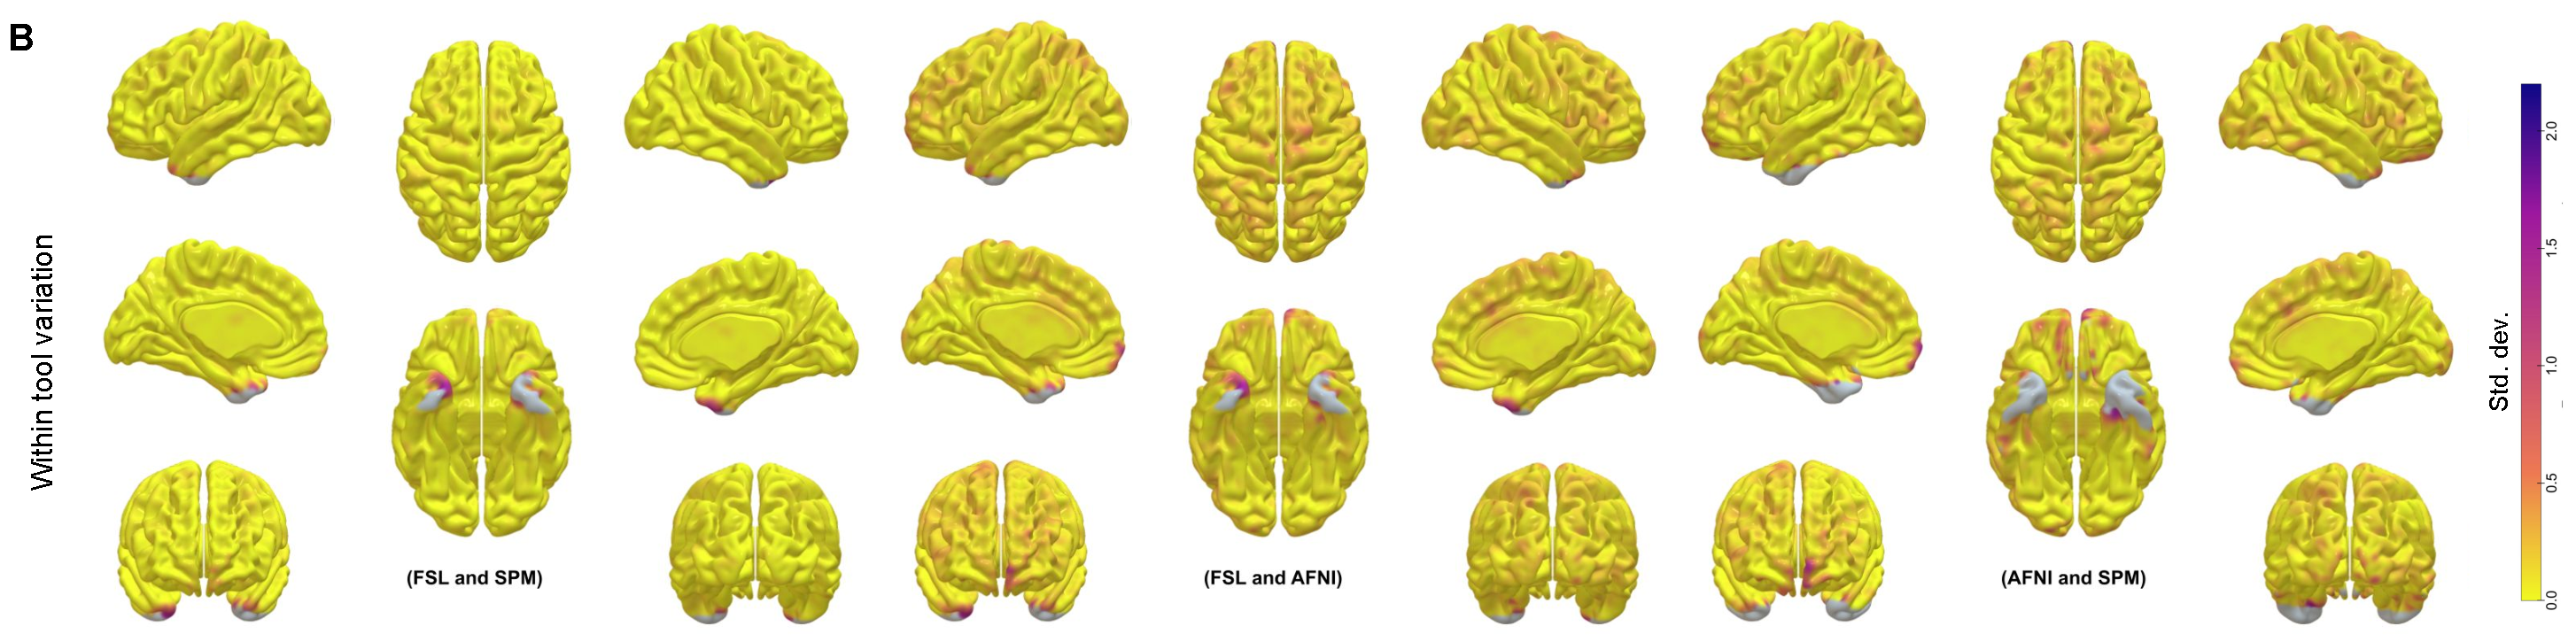
\includegraphics[width=\linewidth]{figures/maps-on-surf-unthresh-fuzzy(std).pdf}
    %\caption{Standard deviation of thresholded t-statistics map on template surface}
    \label{fig:unthresh-varmaps2}
  \end{subfigure}
  \hfill
  \begin{subfigure}[t]{\linewidth}
    \centering
    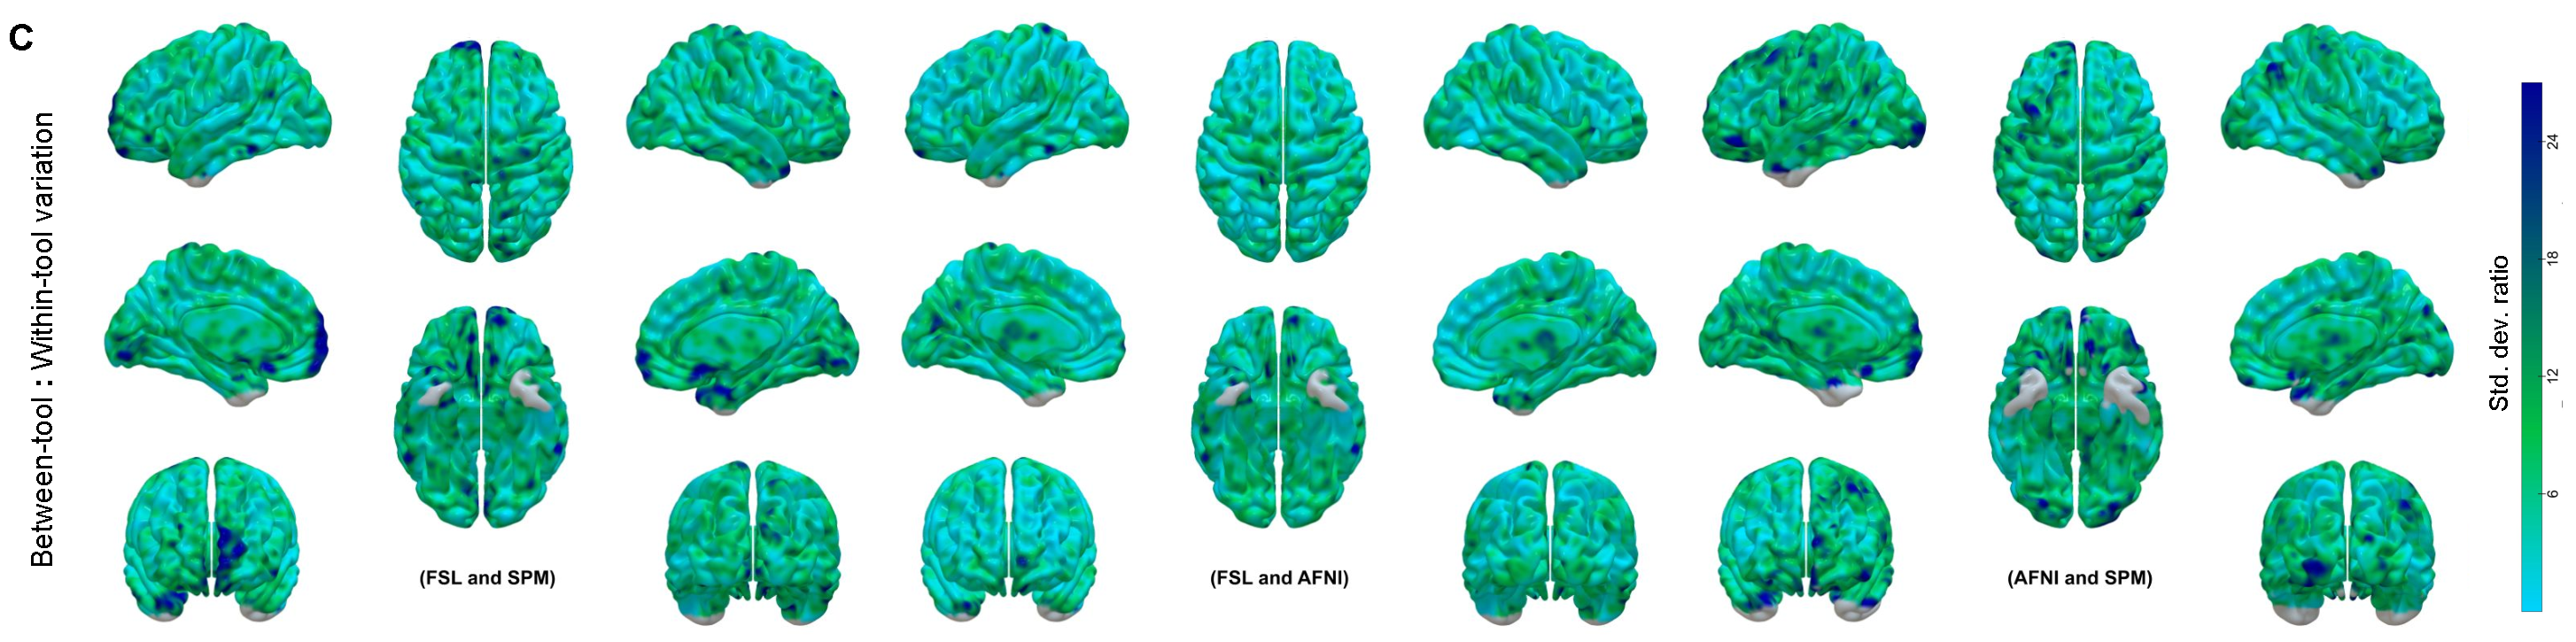
\includegraphics[width=\linewidth]{figures/maps-on-surf-unthresh-ratio(std).pdf}
    %\caption{Standard deviation of thresholded t-statistics map on template surface}
    \label{fig:unthresh-ratio}
  \end{subfigure}
  \caption{Surface maps of standard deviation of unthresholded T-statistics.}
  \label{fig:unthresh-varmaps}
  \end{minipage}}
\end{figure}


The scatter plot in Figure~\ref{fig:correlations} represents the correlation of standard deviation between conditions.
We found three major clusters, including upper, lower, and identity.
The identity cluster corresponds to the correlations between 0.9 and 1.1; the upper cluster shows correlations where BT $\approx$ 0;
and the lower cluster represents correlations where WT $\approx$ 0.
The identity area is also represented on the surface maps in the second row in Figure~\ref{fig:correlations}.
This figure shows the spatial localization of the parts of the brain that are numerically dependent.
We can see regions such as the occipital lobe in the posterior view and the frontal lobe in the interior view 
that are highly correlated in BT and WT results.
This refines the presented results in Figure~\ref{fig:unthresh-varmaps},
which indicates how spatial variabilities are simulated using numerical perturbations in some areas.
% Spatial localization of significant activation in the thresholded images also varied across software packages.
% Moreover, results show that pair of FSL-SPM has the least correlation of variability in within tool and between tool.
% This will implies that ... which can help for further investigations. 


%%%%%%%%%% Corr. plot of tstats%%%%%%%%
\begin{figure}[b]
  \fbox{\begin{minipage}{\dimexpr \textwidth-2\fboxsep-2\fboxrule}
    \begin{subfigure}[t]{\linewidth}
      \centering
      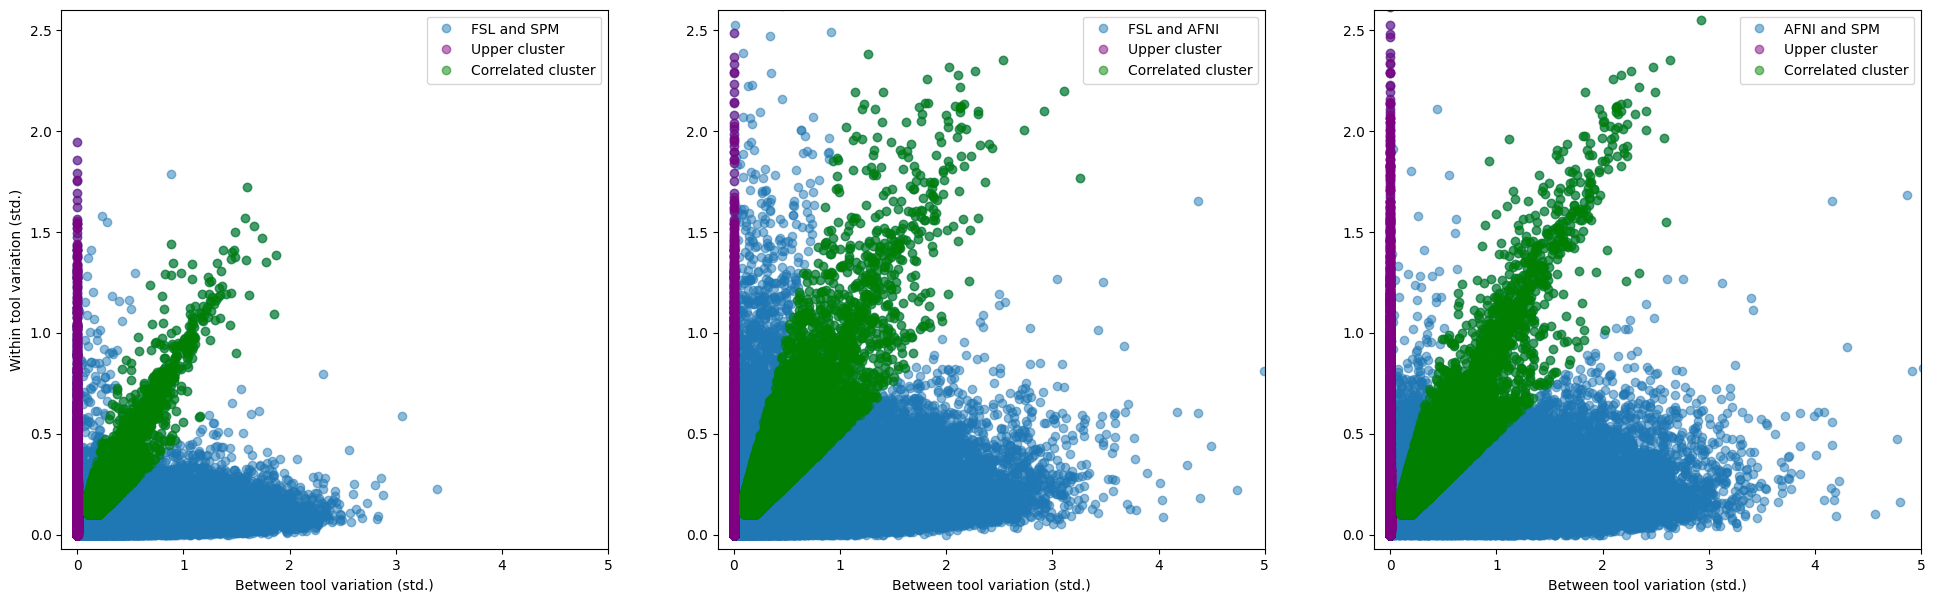
\includegraphics[width=\linewidth]{figures/std-corr-unthresh-plot.png}
      %\caption{Standard deviation of thresholded t-statistics map on template surface}
      \label{fig:unthresh-corrplot}
    \end{subfigure}
    \hfill
    \begin{subfigure}[t]{\linewidth}
      \centering
      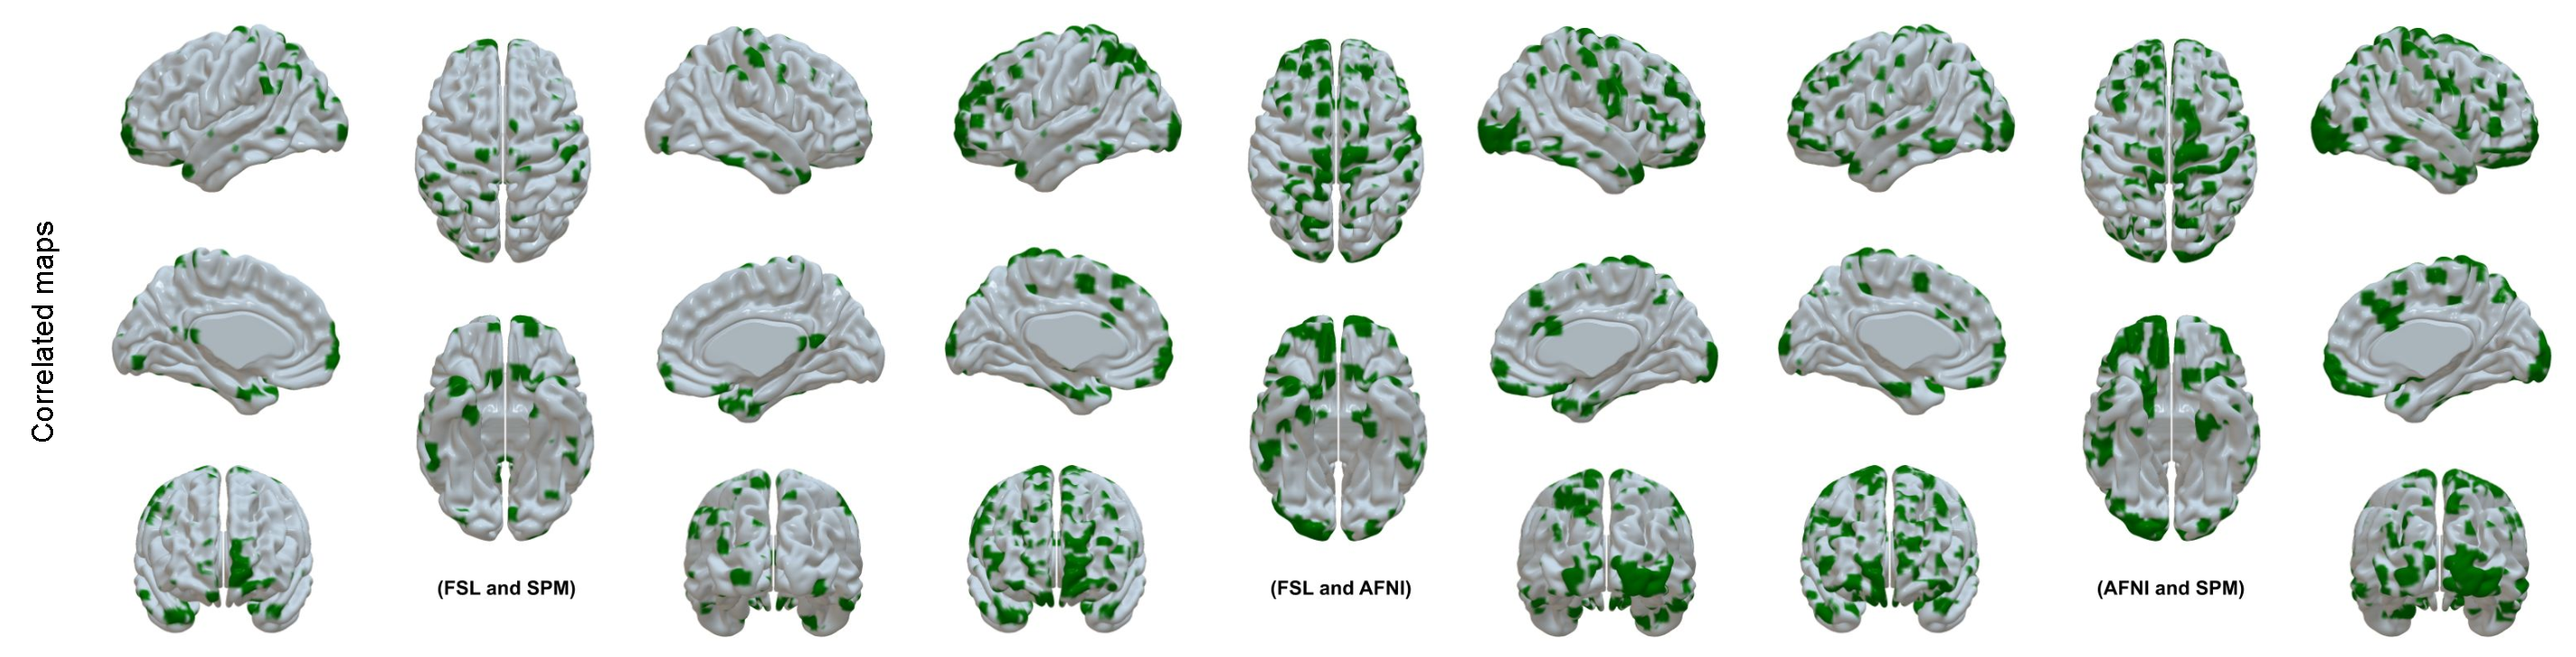
\includegraphics[width=\linewidth]{figures/maps-on-surf-unthresh-tool(corr).pdf}
      %\caption{Standard deviation of thresholded t-statistics map on template surface}
      \label{fig:unthresh-corrmaps}
    \end{subfigure}
  \caption{Correlation of variability in BT and WT variations in unthresholded maps. First row plots the correlations
  voxel by voxel, which is highlighted with different colors for three major clusters including upper cluster (purple color),
  lower cluster (yellow color), and correlated cluster (green color) which are mapped on surface in the second row.}
  \label{fig:correlations}
  \end{minipage}}
\end{figure}

\subsection{Region-based similarity in BT and WT}
In Figure~\ref{fig:dice-thresh}, we compare region-by-region Dice coefficients of
the group level thresholded maps in BT and WT for all pairs of software packages.
This measures the overlap of voxels which assess the spatial similarity between activated maps.
In WT similarity, the Dice values correspond to the average of Dices computed among three
Fuzzy samples for each pair of tools.
Results show that the similarity between tool variations is correlated with the numerical variations,
which implies that similar anatomical regions are activated, and also the topology of the activation patterns
is preserved between results from two types of variations.
% This correlation highly increases when normalizing Dice scores by the region sizes.
% which reduces the effect of small regions.

% This implies that region by region similarity between two type of variations are preserved.
% Results show that similar anatomical regions are activated in both conditions. 
% This plot suggests the similar topologies of the activation patterns in each condition.
% The average of Dice scores range from to 
% FSL-AFNI variations has the most similarity correlations which means that the results of these two tools are more \dots

% In response to the out of border activated voxels can say:
% This is likely due to the fact that SPM consistently had the smallest analysis mask out of the three packages,
% while FSL had the largest. Number of activated voxels prove this fact.


%%%%%%%%%% Dice plot of thresholded tstats%%%%%%%%
\begin{figure}[b]
  \fbox{\begin{minipage}{\dimexpr \textwidth-2\fboxsep-2\fboxrule}
  \centering
  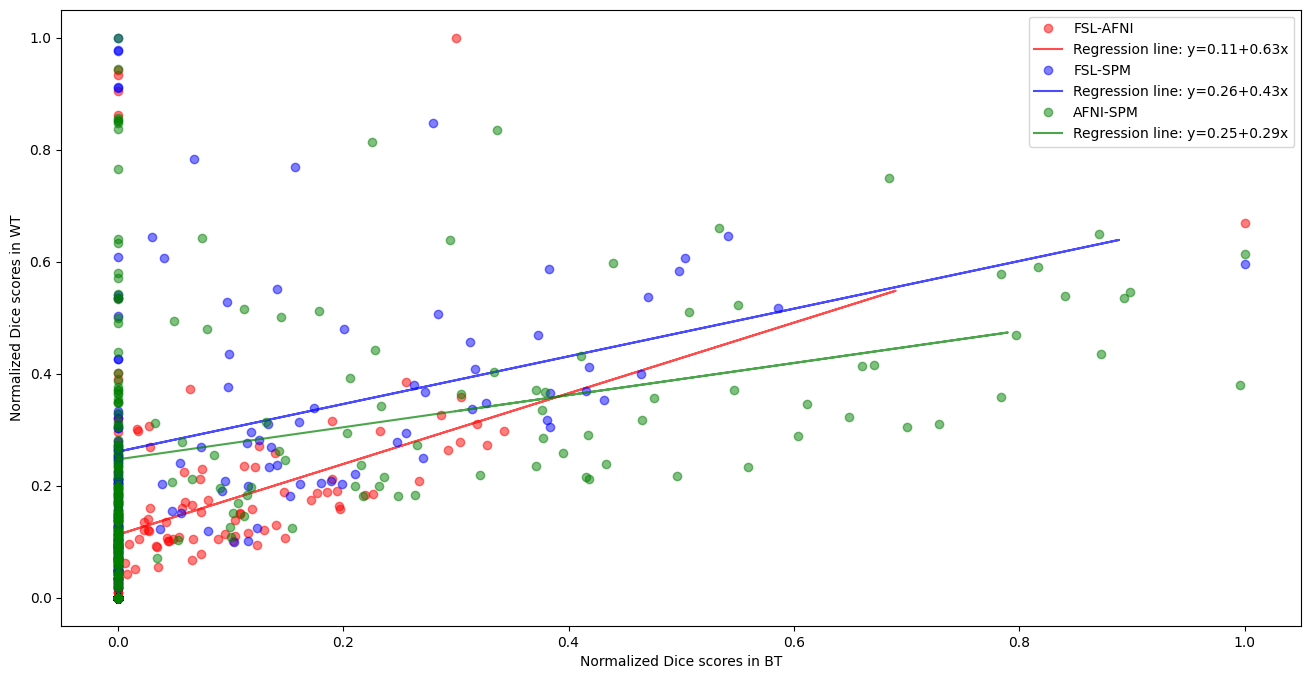
\includegraphics[width=\textwidth]{figures/dices_corr.png}
  \caption{Correlation of Dice coefficients of activated regions between pair of tools and fuzzy samples
  from the thresholded T-statistics. Different pairs are illustrated in different colors. 
  Regression lines are normalized by the region sizes on the right plot.
  Regions correspond to the 360 areas of cortical parcellation (HCP-MMP1.0)~\cite{Glasser-nature}.}
  \label{fig:dice-thresh}
\end{minipage}}
\end{figure}


% %%%%%%%%%% Summary of statstics %%%%%%%%
% \setlength{\tabcolsep}{10pt}
% \begin{table}[h]
%     \centering
%     \begin{tabular}{cccc}
%         \toprule
%         {} & Mean diff. & Std. diff. & Corr. \\
%         \midrule
%         \rowcolor{lightgray}
%         FSL vs. SPM          &  0.242       & 0.534      & 0.599  \\
%         \rowcolor{lightgray}
%         FSL vs. AFNI         &  0.302       & 0.674      & 0.591  \\
%         \rowcolor{lightgray}
%         AFNI vs. SPM         &  0.254       & 0.659      & 0.562  \\
%         Fuzzy FSL and SPM    &  0.00       & 0.00      & 0.00  \\
%         Fuzzy FSL and AFNI   &  0.00       & 0.00      & 0.00  \\
%         Fuzzy AFNI and SPM   &  0.00       & 0.00      & 0.00  \\
%         \bottomrule
%     \end{tabular}
%     \caption{Summary of T-statistics mean and standard deviation of differences and correlation coefficients
%     across three sets of results in two conditions.}
%     \label{table:pipeline-stats}
% \end{table}


% \subsection{The precision that Fuzzy FSL tool can simulate the between tool variations}
% \begin{description}
%   \item[$\bullet$ Figure 5:] Repeat Fig 1-4 for the results of Fuzzy FSL on the precision that simulate mostly betwen tool varions.
% \end{description}

\section{Conclusion \& Discussion}
% In this study, we represented the magnitude of differences in between tool and within tool results.
% Also we showed the numerically dependent parts of the brain, and explained how between tool variations
% are correlated with numerical variability. Moreover, we indicated the spatial similarity between results so that
% numerical perturbations preserve the topology of the avtivation patterns across all three sets of packages in both conditions.

% Further studies can be evaluating the numerical stabilities within tool by focusing on the particular parts of 
% the pipeline that has been identified as the mian sources of variations in~\cite{bowring2019exploring}. 


%
% ---- Bibliography ----
%
% BibTeX users should specify bibliography style 'splncs04'.
% References will then be sorted and formatted in the correct style.
%
\bibliographystyle{splncs04}
\bibliography{biblio}

\end{document}
